\documentclass{standalone}
\usepackage{tikz}
\usetikzlibrary{fit}

\begin{document}
    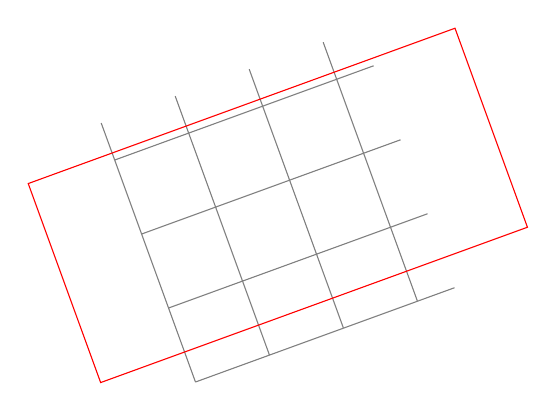
\begin{tikzpicture}[rotate=20]
        \draw[gray,line width=.4pt] (0,0) grid (3.5,3.5);

        \draw[red] (current bounding box.north east) rectangle (current bounding box.south west);
    \end{tikzpicture}

    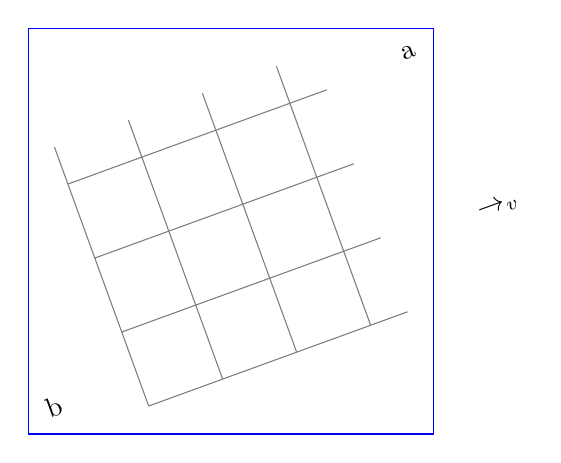
\begin{tikzpicture}[rotate=20]
        \draw[gray,line width=.4pt] (0,0) grid (3.5,3.5);

        \begin{scope}[transform shape]
            % Draw box using nodes and fit
            \node (a) at (current bounding box.north east){a};
            \node (b) at (current bounding box.south west){b};
            \node[  fit=(a)(b),
                    draw=blue,
                    label={[label distance=0.5cm]right:{$\rightarrow_v$}}]{};
        \end{scope}

    \end{tikzpicture}
\end{document}
